\chapter{Implementation}
Make some general points here

\section{Getting Started}

\subsection{Require.js}
When the GatePlay url is visited, the only file downloaded is the main HTML file: index.html. The index then directs the user's browser to download the additional CSS and JavaScript files needed to use GatePlay.

A JavaScript script may used methods or variables defined in the global namespace, even if they were put there by another script. The only restriction is that

\begin{figure}[H]
\begin{lstlisting}[language=html]
<!-- componentview depends on component -->
<!-- Therefore we ensure component is loaded first -->
<script type="text/javascript" src=".../component.js"></script>
<script type="text/javascript" src=".../componentview.js"></script>
\end{lstlisting}
\caption{Example use of Script tags}
\end{figure}

It is time consuming for a human to find and type out a correct ordering for the Script tags, and it would need to be updated every time a file as added or removed, or sometimes if a file were modified.

Require.js is a JavaScript file loader which does automatically loads files in a correct order. Each JavaScript file declares each of its direct dependencies, and Require.js will ensure they are all loaded correctly when the webpage loads.

\begin{figure}[H]
\begin{lstlisting}[language=JavaScript]
// componentview.js

require([
	// Declare the path of each file we require	
	"canvas/model/component"
], function(Component) {
	// Each included file is run, and we can give a name to whatever it returns if desired
	var myComponent = new Component();
	...
});
\end{lstlisting}
\caption{An example file which uses Require.js}
\end{figure}

\section{The Workbench}

GatePlay's workbench is where we create and view circuits. It is implemented using an HTML Canvas element. It is a blank slate which can have shapes and images drawn using the JavaScript API.


\subsection{Fabric.js}
An HTML Canvas only provides low level drawing tools. You are able to draw shapes and images on it, but there is no concept of persist objects on the canvas.

Fabric.js is a library which wraps HTML Canvases with an object model, allowing GatePlay to interact at the level of objects being added to, modified, and remove from the canvas. 

Suppose I wanted to add a rectangle to a canvas, and then move it to a new location. Using Fabric.js this is two library calls (one to add a rectangle object and one to change the position property of the object). Using an HTML Canvas it is still one call to draw the rectangle, but moving it would require calculating what would be behind the rectangle, drawing that over the rectangle, and then re-drawing the rectangle at its new location.

Initially GatePlay used a different canvas framework called KineticJS, but due to difficulties getting features like snap-to-grid working I switched to Fabric.js.

\subsection{MVC with Backbone.js}
Model-view-controller\footnote{http://en.wikipedia.org/wiki/Model-view-controller} is a design pattern to simply program development. GatePlay uses MVC in the implementation of the workbench. MVC applications contain three types of components:

\begin{itemize}
	\item A \textbf{model} which stores some part of the state of the application
	\item A \textbf{view} which displays a representation of one of the models to the user
	\item A \textbf{controller} which processes user input, and updates the appropriate models.
\end{itemize}

\begin{figure}
	\centering
	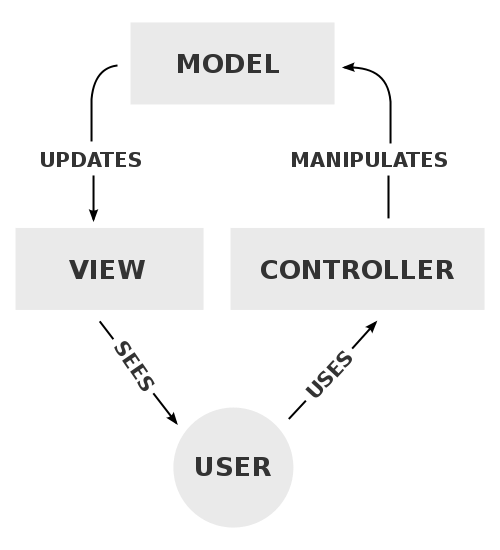
\includegraphics[width=\textwidth * 0.5]{mvc.png}
	\caption{Interaction of MVC Components, from Wikipedia}
	\label{fig:mvc}
\end{figure}

Backbone.js\footnote{http://backbonejs.org} is a JavaScript library to reduce the amount of boilerplate code in developing MVC JavaScript applications.

One model is the Wire model as shown in figure~\ref{fig:wiremodel}. It includes a lot of the same information as the Wire objects used in the simulation, but also includes information regarding the \textit{fixed points} of the wire.

We then create a view associated with the Wire model (figure~\ref{fig:wireview}). 

\begin{figure}
\begin{lstlisting}[language=JavaScript]
Backbone.Model.extend({
	defaults: function() {
    	return {
        	id: nextWireId++,
        	sourceId: -1,
        	sourcePort: -1,
       	 	targetId: -1,
        	targetPort: -1,
        	fixedPoints: [],
        	truthValue: TruthValue.UNKNOWN
    	}
	},
})
\end{lstlisting}
caption{Definition of a Wire model}
\label{fig:wiremodel}
\end{figure}

\begin{figure}
\begin{lstlisting}[language=JavaScript]
Backbone.View.extend({
    initialize: function(options) {
        // When the model is changed, update the view
        this.model.on("change:fixedPoints", this.render, this);
        this.model.on("change:truthValue", this._setWireColor, this);
    },

    render : function() {
        var model = this.model;
		
		// Using the model data we can now draw wires on the canvas
    },

    _setWireColor: function() {
        var truthValue = this.model.get("truthValue");
        
        // We can now re-render the wire with the new colour
    }
});
\end{lstlisting}
caption{Definition of a Wire view}
\label{fig:wireview}
\end{figure}


\subsection{Editing Mode}


\subsection{Running Mode}

\section{The Simulator}
The implementation of GatePlay's simulator is simply a transliteration of the algorithms and ideas explained in section~\ref{chapter:simulation} to JavaScript. The following six classes fully implement the simulator:

\begin{itemize}
	\item \textbf{truthvalue.js} defines constants $True$, $False$, and $Unknown$
	\item \textbf{component.js} defines a Component by its input count, output count, and evaluation function
	\item \textbf{wire.js} defines a Wire by its input component and port, output component and port, and truth value
	\item \textbf{circuitevent.js} defines a CircuitEvent by component, port, timestamp, and value
	\item \textbf{functions.js} contains definitions of all the Evaluation Functions available to the simulator 
	\item \textbf{circuit.js} is the only class which need be visible from outside the simulator. It has an interface to add components and wires. Circuit.js implements the algorithm for the event loop. 
\end{itemize}

\section{Drag and Drop}
One of the requirements of GatePlay was that it be easy to use, and I felt the most natural way to add components to the circuit is to drag them on from the side.

\section{Tying GatePlay Together}

\subsection{application.js}
